\chapter{Simulations}

\section{Simulations}

Two GEANT4 based simulations of the hodoscope were developed in 2011 by Derek Glazier at The University of Edinburgh. The first modelled individual tile and fibre combinations in the hodoscope and the transport of photons through these to the SiPMs. Using this the dimensions, configurations and properties of the tiles and fibres could be adjusted to model and optimise the design of the system. The second simulation modelled the operation of the entire detector in conjunction with the calorimeter to determine their performance working together. Details of the results from the first simulation will be discussed in this section, with further details available in \cite{FTTDR2012}.

\begin{figure}
	\centering
	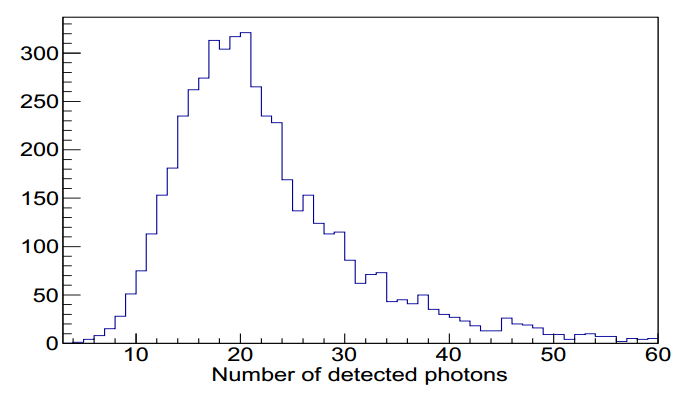
\includegraphics[width=0.9\textwidth]{ImgChap1/mip}
	\caption{Sample results from a validation simulation of the photon output of a MIP in the CLAS inner calorimeter hodoscope. The results matched well with the performance of the detector system. \cite{FTTDR2012} }
	\label{SimulationMIP}
\end{figure}

The simulation determines the energy deposited in the crystals using standard GEANT4 physics models with the properties of the components used (light output, reflectivity, refractive index, etc) inserted to realistically model the detector element design.

The valdity of the simulation was checked by using the same physics to model the CLAS inner calorimeter hodoscope. The output of which is shown in Figure \ref{SimulationMIP} for a MIP, producing a peak of $\sim$18 photoelectrons. This was in good agreement with the performance delivered by the actual detector system.


\subsection{Tile Thickness Simulations}

The amount of energy deposited in a tile by a MIP is proportional to its path length when passing through the scintillator. A thicker tile will result in more photons being released but only a proportion of these will be trapped my the optical fibres. The effect of changing the thickness of the tiles and varying both the number and diameter of optical fibres was simulated, the results of which are shown in Figure \ref{SimulationTileThickness}.


\begin{figure}
	\centering
	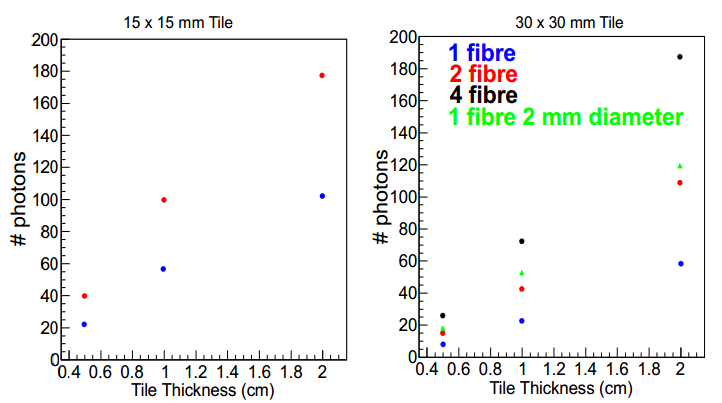
\includegraphics[width=0.9\textwidth]{ImgChap1/tilesim}
	\caption{Simulations of the variation in the photon output of detector tiles with changing thickness and different output fibre configurations. \cite{FTTDR2012}}
	\label{SimulationTileThickness}
\end{figure}

The results show a strong correlation between both increasing tile thickness and number of fibres for both 15x15 mm and 30x30 mm tiles. However there is limited space available for both scintillator and tile routing, so limits must be placed on both. The simulations showed a clear advantage of utilising four 1 mm diameter fibres over one larger 2mm diameter fibre for a 30x30 mm tile, which would occupy a similar volume within the detector.

The simulations indicate that the geometry of the P15 tiles would outperform the larger P30 tiles. A 2 fibre P15 outperforms a 4 fibre P30 at all thicknesses simulated, although the gap closes with increasing tile thickness. However 4 P15s with 2 fibres would require the space for twice as many fibres for the same coverage as 1 P30 with 4 fibres. In addition the smaller tiles would result in a lower acceptance for the detector, with addition space required for reflective materials and unavoidable air gaps between the scintillators. A compromise utilising both designs was selected with a band of P15 tiles surrounding the regions of highest flux at the centre of the detector with the majority of the acceptance covered by the larger P30 tiles. A summary of the simulation results for the performance of the selected thicknesses of the two layers of the detector are shown in Table \ref{SimulationTileThickSummary}.

\begin{table}\centering
	\renewcommand{\arraystretch}{1.3}
	\begin{tabular}{ @{}l  c  c@{}} 
		\toprule
		Tile Type & Thickness & Expected Photons \\
		& {\small [mm]}& \\
		\midrule
		P15 & 7 & 70 \\
		& 15 & 150 \\
		\midrule
		P30 & 7 & 55  \\
		& 15 & 120 \\
		\bottomrule
	\end{tabular}
	\caption{Summary of the expected photon output of the detector tile dimensions selected for use in the hodoscope.}
	\label{SimulationTileThickSummary}
\end{table}

\subsection{Timing Resolution}

Following a similar format to the results for tile thickness, the results for timing resolution are shown in Figure \ref{SimulationTiming}.

\begin{figure}
	\centering
	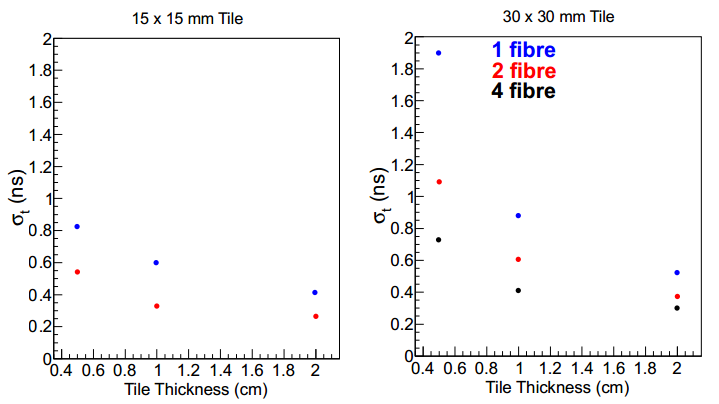
\includegraphics[width=0.9\textwidth]{ImgChap1/timingsim}
	\caption{Results showing how the timing resolution of detector elements varies with thickness and different output fibre combinations. \cite{FTTDR2012}}
	\label{SimulationTiming}
\end{figure}

The critical point to notice is that increasing the number of photons collected improves the timing resolution of the detector elements. The absolute rate of improvement is most significant at lower levels of photon collection, but the effects continues throughout the range of thickness tested in these simulations. The results indicated that sub nanosecond timing resolution is achievable for the detector element design and 0.5 ps levels of timing could be achieved with photon output levels of $\sim$55 photoelectrons. A summary of results for the tiles dimensions used in the construction of the detector are shown in Table \ref{SimulationTileTimingSummary}.

\begin{table}\centering
	\renewcommand{\arraystretch}{1.3}
	\begin{tabular}{ @{}l  c  c  c@{}} 
		\toprule
		Tile Type & Thickness & Expected Photons & Timing Resolution \\
		& {\small [mm]}& & {\small [ns]}\\
		\midrule
		P15 & 7 & 70 & 0.40\\
		& 15 & 150 & 0.30\\
		\midrule
		P30 & 7 & 55 & 0.50\\
		& 15 & 120 & 0.35\\
		\bottomrule
	\end{tabular}
	\caption{Summary of the expected timing resolution of the detector tile dimensions selected for use in the hodoscope.}
	\label{SimulationTileTimingSummary}
\end{table}

\subsection{Fibre Bending}

Light losses due to the bend radius of fibres both within the hodoscope enclosure and while routing through CLAS were also simulated as part of these tests, the results of which are shown in Figure \ref{SimulationBendRadius}. The results matched closely by the results reported by Kuraray to limit the bend radius to no less than 2cm, ideally higher to minimize light losses during transport. 

\begin{figure}
	\centering
	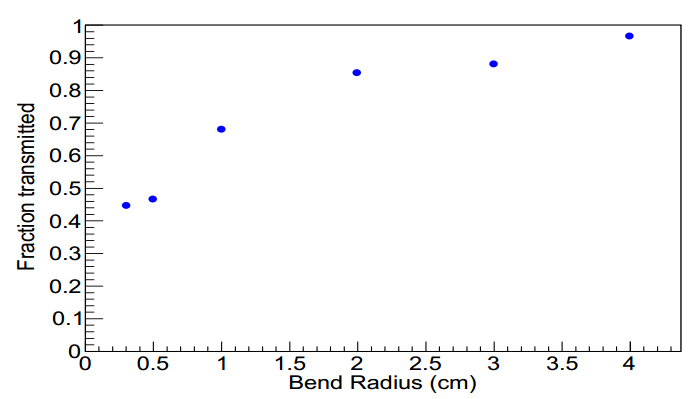
\includegraphics[width=0.9\textwidth]{ImgChap1/bendsim}
	\caption{Results of a simulation measuring the fraction of light loss in a wavelength shifting fibres at different bend radii. \cite{FTTDR2012}}
	\label{SimulationBendRadius}
\end{figure}

\subsection{Radiation Dose}

In addition to the light transport simulations a further study to determine the radiation exposure of the hodoscope was carried out by INFN Genoa. Determining the dose that different elements of the hodoscope would be exposed to ensured they could be suitably resistant and their performance would not degrade significantly over the lifetime of the detector. 
The simulations indicated that without the M\o{}ller shield in place, the largest does would be incurred by the inner pixels of the detector at a rate of 3.8 rad/h. Figure \ref{SimulationRadDose} shows a plot from the INFN simulation, with each pixel representing one of the, 15x15 mm tiles in the calorimeter that is positioned directly behind the hodoscope. 

\begin{figure}
	\centering
	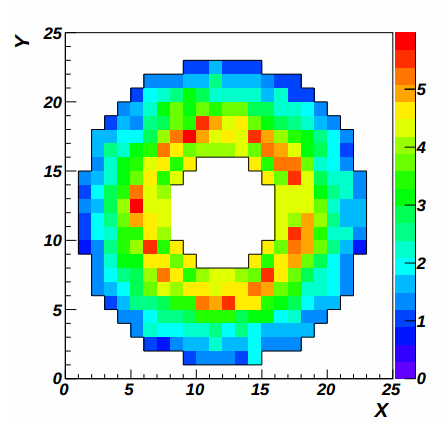
\includegraphics[width=0.9\textwidth]{ImgChap1/raddose}
	\caption{Results from a simulation of the radiation dose experience by the FT-Cal crystals in rad/h at $10^{35}cm^{-2}s^{-1}$ luminosity. Maximum values of just over 5 rad/h were obtained for some of the inner crystals, although averaged over each crystal in the hodoscope this represents a peak of 3.8 rad/h. \cite{FTTDR2012}}
	\label{SimulationRadDose}
\end{figure}

Taking the peak element value of 3.8 rad/h and considering this to be the dose for all elements accross the hodoscope, produces an annual does of 33 krad for each crystal. A large number of studies have shown that exposure to radiation can change the properties of plastic scintillators; reducing the light yield and therefore timing resolution of the tiles. Similar effects have been shown to occur in wavelength shifting fibres and optical cements, reducing their transparency and increasing attenuation length, lowering the performance of the materials.

\textbf{Write a paragraph about literature studies on them, generally done at much higher radiation doses and typically imparted over a much shorter period of time. Studies on the materials used have shown them to be radiation hard to well beyond the expected levels of radiation and much of the damage is expected to be counteracted by annealing processes.}



%Geant4 based simulations were carried out to optimise the design of the detector system. In particular the design of the detector elements was studied as this was the first time such a design had been used before. Keep this short as I wasn't involved in developing, just using this element of the project.

\cite{golovko2008use}

